%% -*- coding: utf-8 -*-
\documentclass[12pt,a4paper]{scrartcl} 
\usepackage[utf8]{inputenc}
\usepackage[english,russian]{babel}
\usepackage{indentfirst}
\usepackage{misccorr}
\usepackage{graphicx}
\usepackage{amsmath}
\usepackage{float}

\usepackage{xcolor}
\usepackage{hyperref}
\hypersetup{colorlinks,
  pdftitle={The title of your document},
  pdfauthor={Your name},
  allcolors=[RGB]{000 000 000}}

\begin{document}
\begin{titlepage}
  \begin{center}

    Санкт-Петербургский политехнический университет Петра Великого

    \vspace{0.25cm}
    
    Институт прикладной математики и механики
    
    Кафедра «Прикладная математика»
    \vfill

	\vspace{0.25cm}
	    Отчёт\\
	по лабораторной работе №3\\
	по дисциплине\\
	«Математическая статистика»

  \bigskip

\end{center}
\vfill

\newlength{\ML}
\settowidth{\ML}{«\underline{\hspace{0.7cm}}» \underline{\hspace{2cm}}}
\hfill\begin{minipage}{0.4\textwidth}
  Выполнил студент\\ В.\,А.~Рыженко\\
\end{minipage}%
\bigskip

\hfill\begin{minipage}{0.4\textwidth}
  Проверил:\\
к.ф.-м.н., доцент\\
Баженов Александр Николаевич\\
\end{minipage}%
\vfill

\begin{center}
  Санкт-Петербург, 2020 г.
\end{center}
\end{titlepage}

\tableofcontents
\listoffigures
\listoftables
\newpage

\section{Постановка задачи}
 
Для 5 распределений:
\begin{itemize}
 \item Нормальное распределение N(x, 0, 1)
 \item Распределение Коши C(x, 0, 1)
 \item Распределение Лапласа L(x, 0, $\frac{1}{\sqrt2}$)
 \item Постановка задач исследованияРаспределение Пуассона P(k, 10)
 \item Равномерное распределение U(x, $-\sqrt{3}, \sqrt{3}$) 
\end{itemize}
 
Сгенерировать выборки размером 20 и 100 элементов.
Построить для них боксплот Тьюки.
Для каждого распределения определить долю выбросов экспериментально (сгенерировав выборку, соответствующую распределению 1000
раз, и вычислив среднюю долю выбросов) и сравнить с результатами,
полученными теоретически.

\section{Теория}

\subsection{Распределения}

\begin{itemize}
\begin{item}
Нормальное распределение
\begin{equation}\label{eq:Normal}
\centering
 N(x, 0, 1) = \frac{1}{\sqrt{2\pi} } e^{-\frac{x^2}2}
\end{equation}
\end{item}

\begin{item}
Распределение Коши
\begin{equation}\label{eq:Cauchy}
\centering
 C(x, 0, 1) = \frac{1}{\pi} \frac{1}{x^2 + 1}
\end{equation}
\end{item}

\begin{item}
Распределение Лапласа
\begin{equation}\label{eq:Laplace}
\centering
L(x, 0, \frac{1}{\sqrt2}) = \frac{1}{\sqrt{2} } e^{\sqrt2|x|}
\end{equation}
\end{item}

\begin{item}
Распределение Пуассона
\begin{equation}\label{eq:Poisson}
\centering
P(k, 10) = \frac{10^k}{k! } e^{-10}
\end{equation}
\end{item}

\begin{item}
Равномерное распределение
\begin{equation}\label{eq:Uniform}
\centering
U(x, -\sqrt{3}, \sqrt{3})  = 
\begin{cases}
\frac{1}{2\sqrt3}, &\mbox{при } |x| \leq \sqrt3 \\ 0 , &\mbox{при } |x| \textgreater \sqrt3
\end{cases}
\end{equation}
\end{item}
\end{itemize}

\subsection{Боксплот Тьюки}
\subsubsection{Определение}

Боксплот (англ. box plot) — график, использующийся в описательной статистике, компактно изображающий одномерное распределение вероятностей.

\subsubsection{Описание}

Такой вид диаграммы в удобной форме показывает медиану, нижний и верхний квартили и выбросы. Несколько таких ящиков можно нарисовать бок
о бок, чтобы визуально сравнивать одно распределение с другим; их можно располагать как горизонтально, так и вертикально. Расстояния между
различными частями ящика позволяют определить степень разброса (дисперсии) и асимметрии данных и выявить выбросы.

\subsubsection{Построение}

Границами ящика служат первый и третий квартили, линия в середине
ящика — медиана. Концы усов — края статистически значимой выборки
(без выбросов). Длину «усов» определяют разность первого квартиля и полутора межквартильных расстояний и сумма третьего квартиля и полутора
межквартильных расстояний. Формула имеет вид

\begin{equation}\label{eq:borders}
\centering
X_1 = Q_1 - \frac{3}{2}(Q_3 - Q_1), X_2 = Q_3 + \frac{3}{2}(Q_3 - Q_1),
\end{equation}

где $X_1$ — нижняя граница уса, $X_2$ — верхняя граница уса, $Q_1$ — первый
квартиль, $Q_3$ — третий квартиль.
Данные, выходящие за границы усов (выбросы), отображаются на графике
в виде маленьких кружков

\subsection{Теоретическая вероятность выбросов}

По формуле ~\eqref{eq:borders}можно вычислить теоретические нижнюю и верхнюю границы уса
($X_1^T$ и $X_2^T$ соответственно).
Выбросами считаются величины $x$, такие что:
\begin{equation}\label{eq:emissions}
\centering
\left[ 
      \begin{gathered} 
       x \textless X_1^T \\
	  x \leq X_2^T \\
      \end{gathered} 
\right.
\end{equation}

Теоретическая вероятность выбросов для непрерывных распределений

\begin{equation}\label{eq:prob1}
\centering
P_B^T = P(x < X_1^T) + P(X > X_2^T) = F(X_1^T) + (1 - F(X_2^T)),
\end{equation}

где $F(X) = P(x\textgreater X) $ - функция распределения. \\

Теоретическая вероятность выбросов для дискретных распределений
\begin{equation}\label{eq:prob2}
\centering
P_B^T = P(x < X_1^T) + P(X > X_2^T) = (F(X_1^T) - P(x = X_1^T)) + (1 - F(X_2^T)),
\end{equation}

где $F(X) = P(x\textgreater X) $ - функция распределения.
\section {Реализация}
Лабораторная работа выполнена с помощью встроенных средств языка программирования Python в среде разработки Visual Code. Исходный код лабораторной работы приведён в приложении.
 
\section{Результаты}
\subsection{Боксплот Тьюки}
\begin{figure}[H]
  \centering
  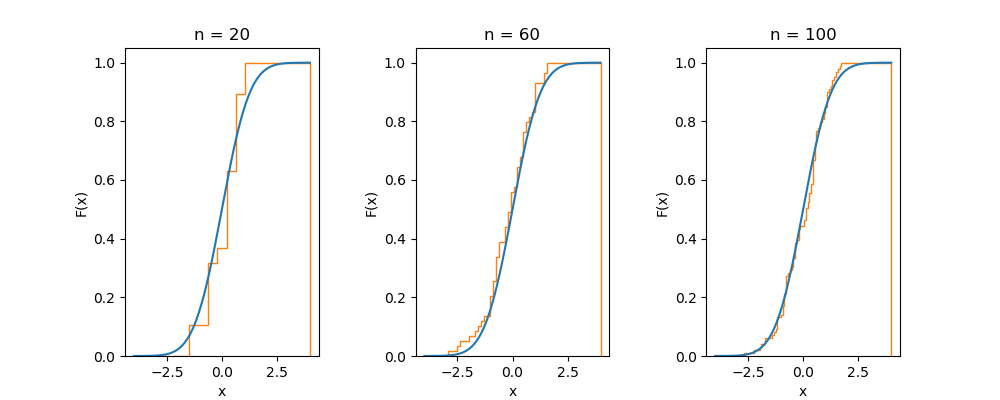
\includegraphics[width=0.8\textwidth]{Normal.png}
  \caption{Нормальное распределение ~\eqref{eq:Normal}}
 
\end{figure}
\begin{figure}[H]
  \centering
  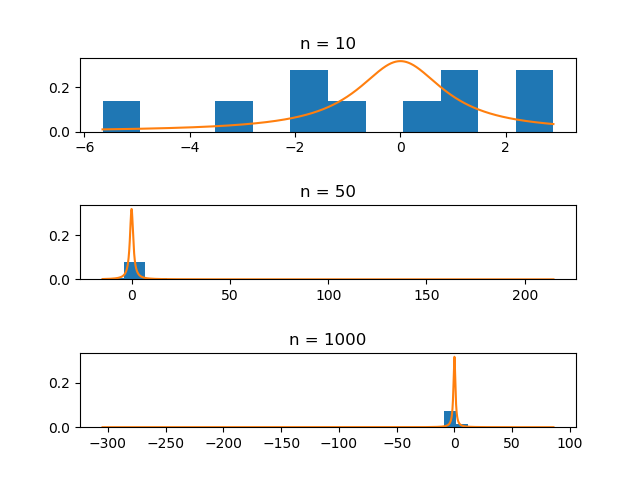
\includegraphics[width=0.8\textwidth]{Cauchy.png}
  \caption{Распределение Коши ~\eqref{eq:Cauchy}}
\end{figure}
\begin{figure}[H]
\centering
  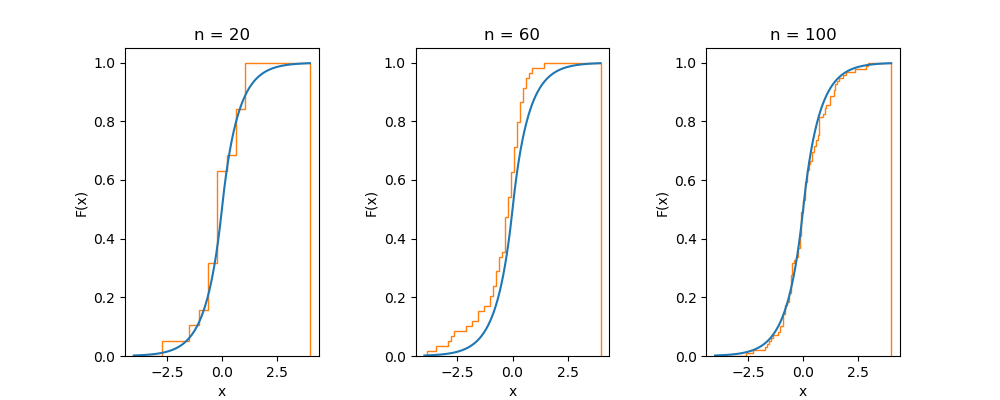
\includegraphics[width=0.8\textwidth]{Laplace.png}
  \caption{Распределение Лапласа ~\eqref{eq:Laplace}}
\end{figure}
\begin{figure}[H]
  \centering
  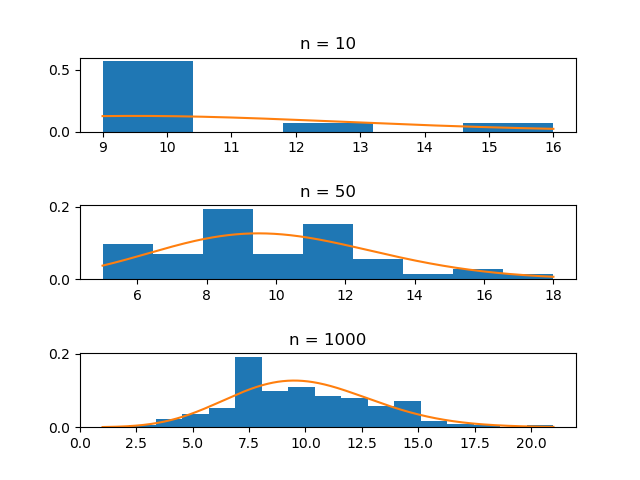
\includegraphics[width=0.8\textwidth]{Poisson.png}
  \caption{Распределение Пуассона ~\eqref{eq:Poisson}}
\end{figure}
\begin{figure}[H]
  \centering
  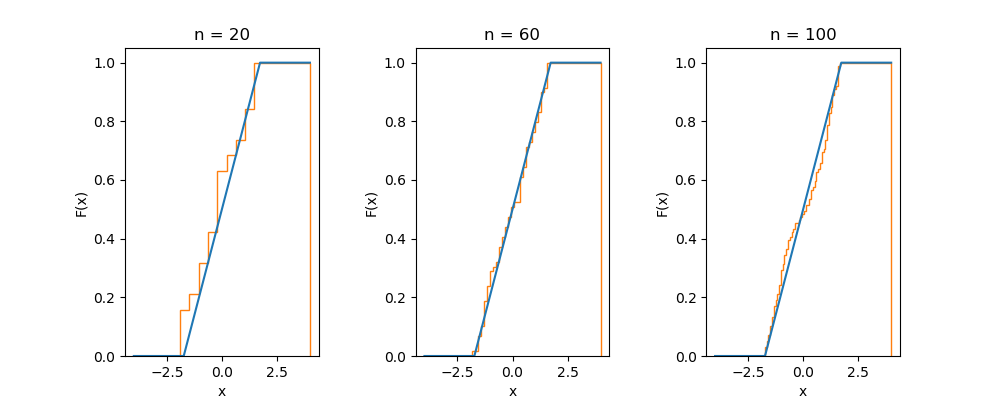
\includegraphics[width=0.8\textwidth]{Uniform.png}
  \caption{Равномерное распределение ~\eqref{eq:Uniform}}
\end{figure}

\subsection{Доля выбросов}

\begin{table}[H]
  \centering
\begin{tabular}{| c | c | c |}
\hline
 Выборка  &   Среднее  & Дисперсия \\
\hline
 Normal, n = 20      &   0.017  & 0.001 \\
\hline
 Normal, n = 100     &  0.0095 & 0.0001 \\
\hline
 Cauchy, n = 20      &  0.139 & 0.005\\
\hline
 Cauchy, n = 100     &  0.154 & 0.001\\
\hline
 Laplace, n = 20     &  0.065 & 0.004\\
\hline
 Laplace, n = 100    & 0.0642 & 0.0009 \\
\hline
 Poisson, n = 20     &  0.016 & 0.002\\
\hline
 Poisson, n = 100    &  0.0101 & 0.0003\\
\hline
 Uniform, n = 20     & 0 & 0 \\
\hline
 Uniform, n = 100    &  0 & 0 \\
\hline
\end{tabular}
  \label{table:EjectionsProportion}
\caption{Доля выбросов}
\end{table}

\subsection{Теоретическая вероятность выбросов}

\begin{table}[H]
  \centering
\begin{tabular}{| c | c | c | c | c | c |}
\hline
Распределение  & $Q_1^T$ & $Q_3^T$ & $X_1^T$ & $X_2^T$ & $P_B^T$~\eqref{eq:prob1}~\eqref{eq:prob2}\\
\hline
Нормальное распределение & -0.674 & 0.674 & -2.698 & 2.698 & 0.007 \\
\hline
Распределение Коши & -1  & 1 & -4 & 4 & 0.156 \\
\hline
Распределение Лапласа & -0.490 & 0.490 & -1.961 & 1.961 & 0.063 \\
\hline
Распределение Пуассона & 8 & 12 & 2 & 18 & 0.008 \\
\hline
Равномерное распределение & -0.866 & 0.866 & -3.464 & 3.464 & 0 \\
\hline
\end{tabular}
  \label{table:TeorProb}
\caption{Теоретическая вероятность выбросов}
\end{table}

\section{Обсуждение}
Из полученных данных видно, что средняя доля выбросов (для 1000 эксперементов) стремится к теоретической оценке при увеличении размера выборки, для всех распределений, кроме распределения Пуассона~\eqref{eq:Poisson}. Дисперсия в свою очередь стремится к нулю уже для всех распределений. Также можно заметить, что для равномерного распределения отсутвуют выбросы, а вероятность их появления равна 0.

\section{Приложения}
Репозиторий на GitHub с релизацией: \href{https://github.com/WiillyWonka/MatStat}{github.com}.
\end{document}
